\section{Neural networks}

An Artificial Neural Network (ANN) is a processing system made from large number of interconnected simple processing elements - neurons. Architecture ANNs was inspired by structure of biological brain - both brain and ANN process information similarly and learns from examples.

This creates different approach to problem solving compared to conventional computing. Instead of predictable algorithmic approach, ANNs allows solving problems without understanding of problem, but with lower accuracy. \cite{history}

\subsection{History}

In 1943 neurophysiologist Warren McCulloch and mathematician, Walter Pitts developed first model of ANN. Neurons in their models had fixed threshold and were able to simulate simple logic functions. \citep{history}

\begin{figure}[h]
\centering
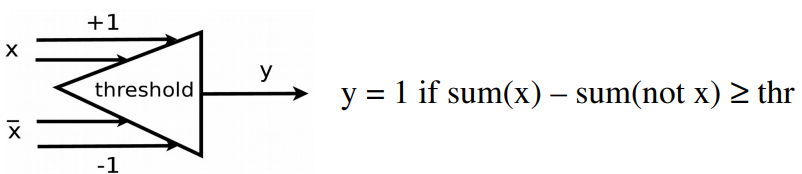
\includegraphics[width=0.9\textwidth]{images/firstneuron.png}
\caption{Model of an artificial neuron according to McCulloch and Pitts \cite{NNFarkas}}
\end{figure}

After initial period of enthusiasm and few other contributions to the field, period of frustration followed. During that time there were only few researchers continued work on solving problems with neural networks. During this time Klopf developed basis for learning and Werbos developed back-propagation algorithm.

This period lasted up to the 1980s, when multiple new contributions renewed wider interest.Hopfield described recurrent neural networks and presented paper \textit{Neural Networks and Physical Systems with Emergent Collective Computational Abilities}.\citep{history}

Neural networks become recently much more publicly know, caused by advances in computing power allowing much bigger number of neurons. It allowed for much more complex tasks as image generation from natural language prompts or chatbots capable of deeper conversations.

\subsection{Different models of neural networks}

There are hundreds of different models and architectures of neural networks with different advantages and disadvantages for different purposes. Some of the most used architectures are:

\begin{itemize}
    \item Single perceptrons
    \item Multi-layer perceptrons
    \item Convolutional neural network
    \item Recurrent neural network
    \item Self-Organizing Maps
    \item Radial Basis Function Network
    \item Hopfield autoassociative memory
\end{itemize}

In practise, multiple architectures are often combined to achieve desired outcome.\citep{NNFarkas}

\subsubsection{Simple perceptron}
It was proposed in 1958 by American psychologist, F. Rosenblatt. It is more general model, with free parameters, stochastic connectivity and threshold elements.\citep{NNFarkas}

\begin{figure}[h]
\label{simplePer}
\centering
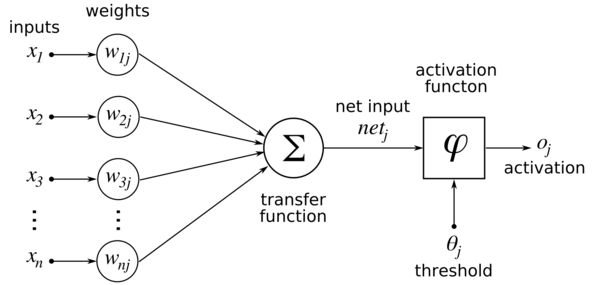
\includegraphics[width=0.7\textwidth]{images/simpleneuron.png}
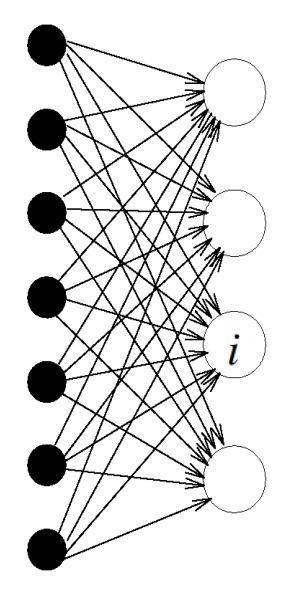
\includegraphics[width=0.2\textwidth]{images/simplelayer.png}
\caption{Model of simple perceptron and layer of simple perceptrons \cite{NNFarkas}}
\end{figure}

Activation of this perceptron consists of weighted sum of inputs, from which we subtract threshold $\theta$ (\ref{act1}). Result is then run through activation function, either uni/bipolar for discrete perceptron or sigmoid for continuous perceptron. In practise, threshold is expressed as another weighted input $x_{n+1}$, with static value of -1, commonly called bias(\ref{act2}).

\begin{equation}
\label{act1}
o_j = f(\sum_{i=1}^n w_{ij}x_i - \theta_j)
\end{equation}
\begin{equation}
\label{act2}
o_j = f(\sum_{i=1}^{n+1} w_{ij}x_i)
\end{equation}

Learning rule for adjust weights in discrete perceptron:
\begin{equation}
\label{learn1}
w_j(t+1) = w_j(t) + \alpha(d - y)x_j
\end{equation}

And for continuous perceptrons:
\begin{equation}
\label{learn2}
w_j(t+1) = w_j(t) + \alpha(d^{(p)} - y^{(p)})f'x_j
\end{equation}

Where $\alpha(Alpha)$ represents learning rate.

Simple perceptron can solve only lineary separable classes. This caused loss of interest in neural networks in many researchers 1970s as many real problems are lineary non-separable, thus simple perceptron cannot be used to solve them.

\subsubsection{Multi-layer perceptron}
Multi-layer perceptron(MLP) is probably one of most used architectures today. It is generalisation of simple perceptrons and it contains additional hidden layers. MLP originates from \textit{Rumelhart \& McClelland: Parallel distributed processing} but was earlier described by Werbos in 1974. It is response to critique on perceptrons.\cite{NNFarkas}

In MLP Activations are similar to activations in simple perceptron. Their distinction comes from addition of hidden layers and additional weights. Due this change, output layer is calculated from hidden layer, instead of inputs.

\begin{equation}
\label{act3}
h_k = f(\sum_{j=1}^{n+1} v_{kj}x_j)
\end{equation}
\begin{equation}
\label{act4}
y_i = f(\sum_{j=1}^{q+1} w_{ik}h_k)
\end{equation}

\begin{figure}
\label{multiNet}
\centering
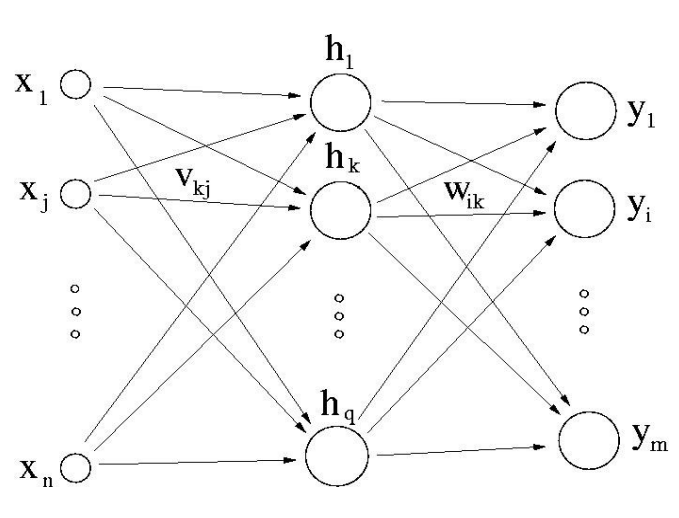
\includegraphics[width=0.7\textwidth]{images/multineuron.png}
\caption{Model of multi-layer neural network \cite{NNFarkas}}
\end{figure}

Activation functions on hidden layers doesn't have similar constrains as output function, but linear function should not be used, as it doesn't add any depth to network. Common activation functions are sigmoid or hyperbolic tangent function.

Learning of MLP uses back-propagation algorithm with different equations for hidden and output layers. Weight adjustments are calculated backwards from output layers to the first hidden layer.\cite{NNFarkas}

Equation for calculating Hidden-output weights:

\begin{equation}
\label{learn3}
w_{ik}(t+1) = w_{ik}(t) + \alpha\delta_ih_k\text{ where }\delta_i = (d_i-y_i)f'_i
\end{equation}

And for Input-hidden weights:
\begin{equation}
\label{learn4}
v_{kj}(t+1) = v_{kj}(t) + \alpha\delta_kx_j\text{ where }\delta_k = (\sum_iw_{ik}\delta_i)f'_k
\end{equation}

\subsection{Creating neural networks}

To successfully create a neural network for accurate classification or prediction tasks, three key components play major role: high-quality dataset, the selection of an appropriate neural network model, and the identification of optimal hyperparameters for the training process itself.

\subsubsection{Training process}

During training, model iterates through dataset, predict outcome and calculates weight changes based on error. One such iteration is called \textbf{epoch}.

One training iteration usually consist of these steps:
\begin{itemize}
  \item for each input $x$ and desired output $d$ (in random order)
  \begin{enumerate}
    \item compute output: $y=?(Wx)$
    \item compute error: $e=d-y$
    \item compute adjustment: $\Delta W =?(W,x,y,e)$
    \item adjust weights:$\Delta W(t+1)=W(t)+\alpha\Delta W$
  \end{enumerate}
\end{itemize}

This iteration continues until certain stopping criteria is meet, usually number of passed epochs or accuracy of model.

This is also called \textit{sequential training}. Other used type of training is called \textit{batch training}. In batch, instead of iterating through input-output pairs is everything calculated in parallel. This is done through matrix multiplication and can significantly speed up calculations, at cost of higher memory requirement and harder implementation.\cite{NNFarkas}

\subsubsection{Datasets}

Selection of proper dataset is crucial for training process - dataset should properly represent data from problem. In practise, getting ideal datasets is complicated and often impossible and contain too small sample of data. This can be partially corrected by using data augmentation. 

Data augmentations refers to changing available dataset to better suit task needs or generating new data based on present one. As example, in article \textit{Improving handgun detection through a combination of visual features and body pose-based data} \cite{handgun}, authors edited original dataset of high quality images by editing lighting and "zooming out" to make humans on them appear smaller \ref{cctv}. This changes simulated of CCTVs, that often cover poorly lit big areas. They also used generation of new data by flattening 3D pose data to 2D from multiple points of view \ref{pose}.

\begin{figure}
\centering
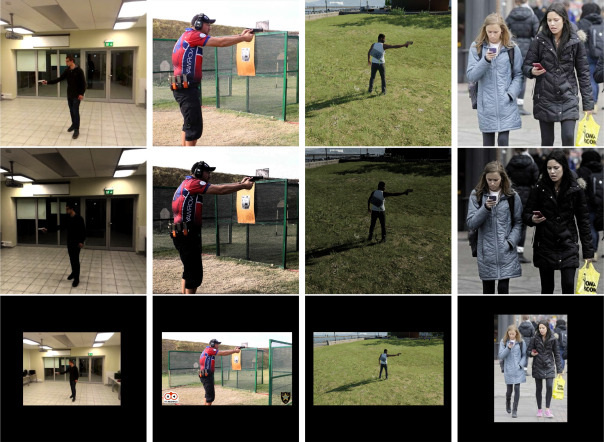
\includegraphics[width=0.7\textwidth]{images/dataaug1.jpg}
\caption{Unedited and edited images \cite{handgun}}
\label{cctv}
\end{figure}

\begin{figure}
\centering
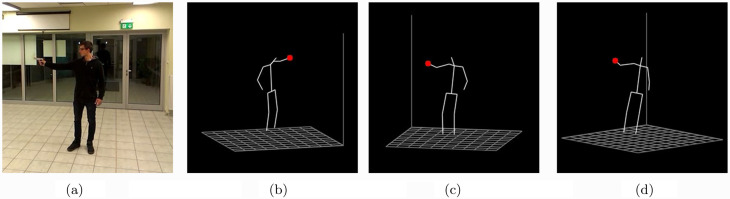
\includegraphics[width=0.7\textwidth]{images/dataaug2.jpg}
\caption{Different points of view \cite{handgun}}
\label{pose}
\end{figure}


